\documentclass[10pt]{beamer}
%\usetheme[
%%% option passed to the outer theme
%    progressstyle=fixedCircCnt,   % fixedCircCnt, movingCircCnt (moving is deault)
%]{}
  
% If you want to change the colors of the various elements in the theme, edit and uncomment the following lines

% Change the bar colors:
%\setbeamercolor{Feather}{fg=red!20,bg=red}

% Change the color of the structural elements:
%\setbeamercolor{structure}{fg=red}

% Change the frame title text color:
%\setbeamercolor{frametitle}{fg=blue}

% Change the normal text color background:
%\setbeamercolor{normal text}{fg=black,bg=gray!10}

%-------------------------------------------------------
% INCLUDE PACKAGES
%-------------------------------------------------------

\usepackage[utf8]{inputenc}
\usepackage[italian]{babel}

%-------------------------------------------------------
% DEFFINING AND REDEFINING COMMANDS
%-------------------------------------------------------

\usetheme{Frankfurt}

%-------------------------------------------------------
% INFORMATION IN THE TITLE PAGE
%-------------------------------------------------------

\title[] % [] is optional - is placed on the bottom of the sidebar on every slide
{ % is placed on the title page
      \textbf{Arbitrary Fault-Tolerant and Locality-Aware MapReduce}
}

\subtitle[]
{
      \textbf{Sistemi Distribuiti e Cloud Computing 2018-2019}
}

\author[Andrea Graziani - 0273395]
{      Andrea Graziani - 0273395 \\
      {}
}

\institute[]
{
      Università degli Studi di Roma “Tor Vergata” \\
      FACOLTA' DI INGEGNERIA \\
      Corso di Laurea Magistrale in Ingegneria Informatica
  
  %there must be an empty line above this line - otherwise some unwanted space is added between the university and the country (I do not know why;( )
}

\date{\today}

%-------------------------------------------------------
% THE BODY OF THE PRESENTATION
%-------------------------------------------------------

\begin{document}

%-------------------------------------------------------
% THE TITLEPAGE
%-------------------------------------------------------

{% % this is the name of the PDF file for the background
\begin{frame}[plain,noframenumbering] % the plain option removes the header from the title page, noframenumbering removes the numbering of this frame only
  \titlepage % call the title page information from above
\end{frame}}

\section{System Architecture}

\begin{frame}[fragile]{System Architecture}{}

\begin{figure}[h]
  \centering
  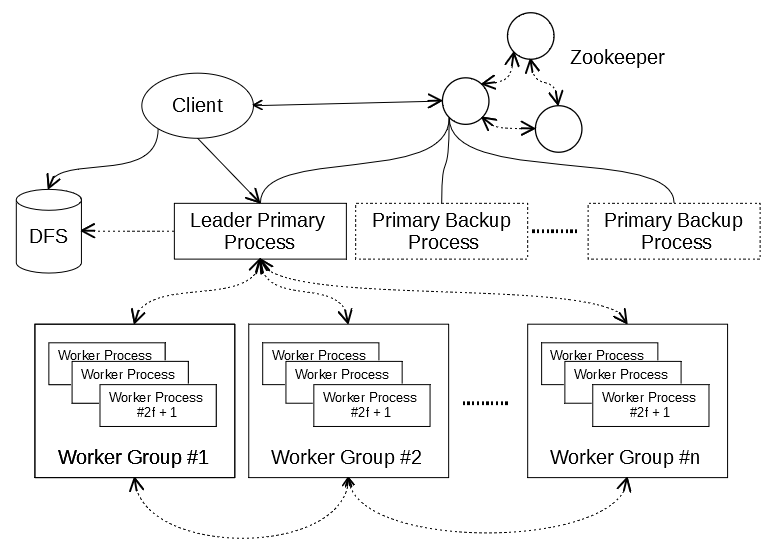
\includegraphics[width=\linewidth]{./images/Architecture.png}
  \caption{System Architecture}
\end{figure}
\end{frame}

% ************************************************************************** %

\subsection{System's processes}

\begin{frame}{System Architecture}{}

\begin{itemize}

\item What assumptions we have made?

\item We distinguish three process types: 
\vspace{10pt}
\begin{itemize}
\item \textit{Client Process}
\item \textit{Primary Process} (PP) 
\item \textit{Worker Process} (WP)
\end{itemize}
\vspace{10pt}

\item How we made the system fault tolerant? What kind of fault tolerance can be achieved with this design?
\item What kind of semantics do we have adopted?
\item Is our system scalable?
\item Our system can be elastic? \textbf{Yes... but}
\item What are the advantages/disadvantages of our solution?
\end{itemize}
\end{frame}

% ************************************************************************** %
\section{System features}


\subsection{Locality-And-State-Aware Deferred Execution} 

\begin{frame}{System features}{Deferred Execution}

\begin{itemize}
\item By default our system is design to use the \textit{Deferred Execution} approach during task scheduling.

\vspace{10pt}
\begin{itemize}
\item What's meant by deferred execution and how it works?

\item What are the advantages of this approach? And the disadvantages?

\item What happens if LPP/WPs crashes?

\item Why \textit{Locality-Aware}?

\item Why \textit{State-Aware}?
\end{itemize}
\vspace{10pt}
\end{itemize}
\end{frame}

\subsection{Speculative Execution}

% ************************************************************************** %
\begin{frame}{System features}{Speculative Execution}

\begin{itemize}

\item In order to improve system's performance we have adopt an approach based on the so called \textit{Speculative Execution}
\vspace{10pt}
\begin{itemize}
\item What's meant by speculative execution? How it works?

\item What happens if the input used during Reduce-Phase is detected as incorrect?

\item What happens if LPP/WPs crashes?
\end{itemize}
\vspace{10pt}
\item Can we do better? \textbf{Yes...but...}
\end{itemize}

\end{frame}

\subsection{Data-Locality-Aware Reduce Scheduling and Shuffle}

% ************************************************************************** %
\begin{frame}{System features}{Data-Locality-Aware Reduce Scheduling and Shuffle}

\begin{itemize}

\item Our system is designed to schedule reduce task considering data locality in order to reduce the overall amount of transferred data between WPs: this approach is called \textit{Data-Locality-Aware Reduce Scheduling}.
\vspace{10pt}
\begin{itemize}

\item "\textit{Moving computation towards data is cheaper than moving data towards computation}".
\item How it works?


\end{itemize}

\end{itemize}

\end{frame}

\subsection{Other features}

% ************************************************************************** %
\begin{frame}{System features}{Other features}

\begin{itemize}
\item Digest output.
\item Leader election and crash failure detection based on Apache Zookeeper.
\end{itemize}

\end{frame}

\begin{frame}[plain,noframenumbering]
  Grazie per l'attenzione!
\end{frame}


\end{document}